\documentclass[a4paper]{article}

\usepackage[utf8]{inputenc}
\usepackage{erk}
\usepackage{times}
\usepackage{graphicx}
\usepackage[top=22.5mm, bottom=22.5mm, left=22.5mm, right=22.5mm]{geometry}

\usepackage[slovene,english]{babel}
\usepackage{hyperref}
\usepackage{url}

\let\oldfootnotesize\footnotesize
\renewcommand*{\footnotesize}{\oldfootnotesize\scriptsize}

\begin{document}
\title{POROČILO IZDELAVE IGRE - AIRBORNE \\
 Računalniška grafika in tehnologija iger, FRI 2022}

\author{Luka Uranič$^{1} (63200035)$, Alen Kurtagić$^{1} (04200012)$,  Ana Maurič$^{1} (64190013)$, \\ Anja Jerala$^{2}$,  Nika Črne$^{2}$} % use ^1, ^2 for author(s) from different institutions

\affiliation{	$^{1}$Univerza v Ljubljani, Fakulteta za računalništvo in informatiko \\ 
				$^{2}$Univerza v Ljubljani, Naravoslovnotehniška fakuteta}

%\email{E-pošta: ciril.bohak@fri.uni-lj.si}

\maketitle

\selectlanguage{slovene}

\begin{abstract}{Abstract}%done
Airborne je letalska igra, narejena v WebGL-ju. Idejo za igro je v tej skupini podal Alen, navdušila ga je letalska tekmovalna igra Air Wars 3 in podobni seminarji pri RGTI-ju iz prejšnjih let. Ker nam je bila ideja drugim članom všeč, smo jo uporabili, razvili in nadgradili v končni izdelek. Ko smo se združili še z oblikovalkama iz NTF-ja, smo idejo tudi malce spremenili glede na njune želje in predloge. Želeli smo ustvariti interaktvino, zanimivo igro, ki bi igralca pritegnila z napetim dogajanjem, realistično sceno in pa tudi lepo vizualno podobo. Delo je bilo razdeljeno na dva osnovna dela: oblikovanje in izvoz modelov (letala in ostalih modelov sveta) v Blenderju ter potem programiranje igre v WebGL-ju. Pomagali smo si z materialom iz vaj in tutoriali na Youtube-u od kreatorja Andrew-a Adamsona. \footnote{\url{https://www.youtube.com/playlist?list=PLPbmjY2NVO_X1U1JzLxLDdRn4NmtxyQQo}}. Celotno delo je trajalo približno 1 mesec. 
\begin{center}
     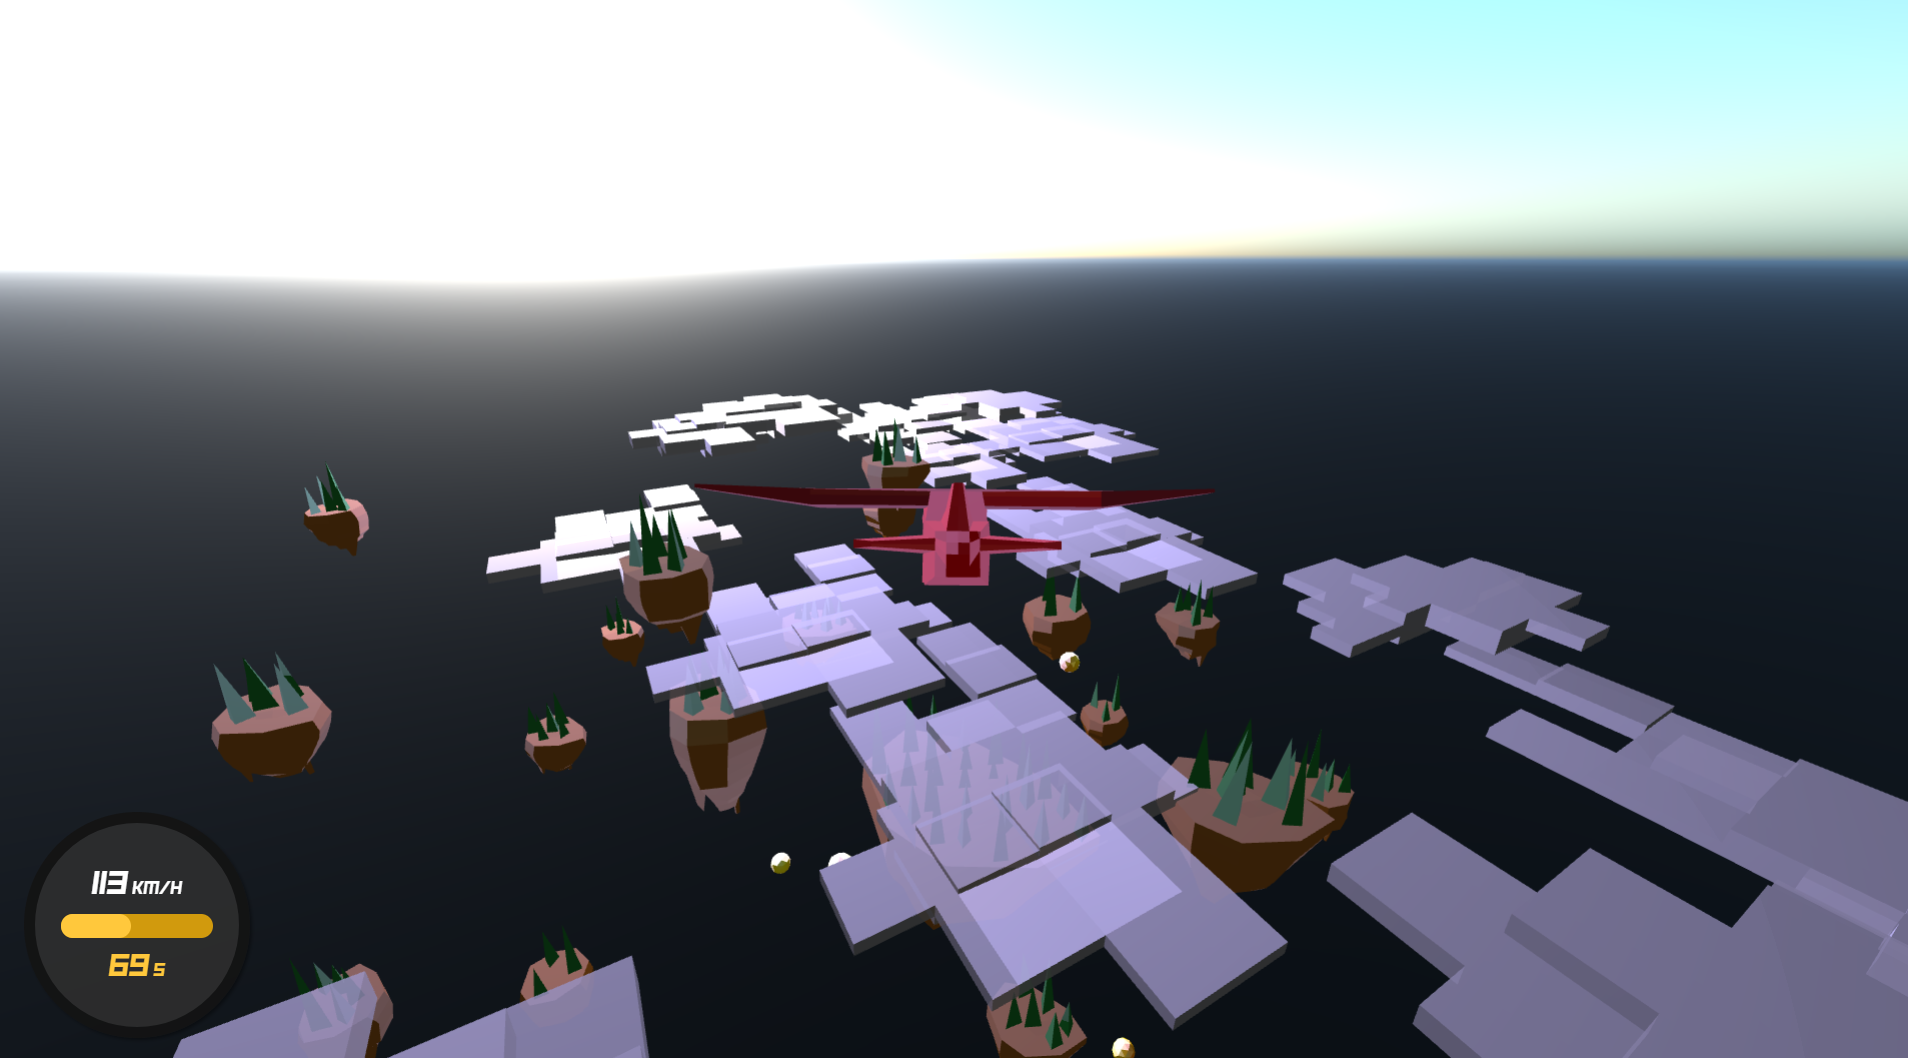
\includegraphics[width=\columnwidth]{igra.jpg}
\end{center}
\end{abstract}

\section{Pregled igre}%done
Igra Airborne je letalska igra iz perspektive 3. osebe. Igralec oz. pilot usmerja letalo, s katerim poskuša nabrati žetone, ki mu povečujejo količino goriva. Igre je konec, ko se letalo zaleti v ovire v svetu ali pa ko mu zmanjka goriva. Igralec mora biti dovolj spreten, da se približa žetonom in jih pobere, brez da se zaleti v ovire, ki so postavljene blizu žetona, medtem ko letala ne more ustaviti, le usmerja po xyz osi sveta - zato je zahtevnost igre srednje zahtevnosti. Namenjena je vsem, ki si jo želijo igrati, tako izkušeni igralci kot tudi začetniki. Letalo se nahaja v zraku, okrog njega porazdeljeno po svetu so lebdeči otoki, oblaki in zlati žetoni, v ozadju je sončno obzorje. Cilj igre je preživeti oz. leteti čim dlje časa, pobrati čim več žetonov. Igralec lahko raziskuje svet po vseh smereh neba.

\subsection{Opis sveta}%done
Naš 3D svet je upodobljen s preprostimi (low-poly) 3D modeli, vendar je njegova podoba še zmeraj realistična. Letalo se lahko premika kamorkoli po xyz smereh. Svet vsebuje rjave lebdeče otoke, na katerih rastejo zelena drevesa, zlate žetone okoli teh otokov in bele prozorne oblake na nebu. V daljavi v neskončnosti se vidi sončno obzorje.

\subsubsection{Pregled}%done
Glaven model v svetu je letalo. Letalo vidi iz 3. perspektive, nahaja se malo za njim, da ima pregled nad vsem okoljem pred in ob letalu. Igralec in letalo se ves čas igre nahajata na sredini zaslona. S pilotiranjem letala se igralec potem obrača naokoli, se približuje in oddaljuje otokom, žetonom, oblakom in ozdaju. Da je letenje bolj prijetno s pomočjo linearne interpolacije premikamo kamero proti določenem offsetu, ki konkretno znaša (-10, 0, 0).

\subsubsection{Ozadje}%done
V ozadju se nahaja sonce, katerega smo vzeli iz vaj. Sonce je nazačetku srednje visoko, na to pa se skozi igro začne spuščati, in igralci, ki so dovolj uspešni, da preletijo vsaj 80s, lahko (kot nagrado) vidijo sončni zahod. 

\subsubsection{Ključne lokacije}%done
Ključna lokacija v svetu je sredina, kjer se nahaja kar nekaj lebdečih otokov. Samo na tej lokaciji lahko igralec najde žetone, za letalo predstavlja nahajališče dobrin, ostalo je samo ozadje - kot je podrobneje opisano v prejšnjem razdelku, to sta ne-interaktivno sončno obzorje in tla.

\subsubsection{Velikost}%done
Svet je srednje velik. Vsebuje približno 20 otokov. Na ta svet gledamo iz 3. perspektive, da si ga lahko v celoti ogledamo in obiščemo. 

\subsubsection{Objekti}%done
Vsi modeli, ki sestavljajo naš svet, so narejeni v Blenderju, v sami kodi pa so uporabljeni kot Gltf modeli. Naredila jih je članica oblikovalka Anja. Zasnovali smo jih kot preproste modele, da bi bil rendering igre še vedno kolikor toliko optimalen, ki pa so še vedno zanimivi na pogled. Ozadje pa sestavljajo objekti, v celoti narejeni v WebGL-u. Modeli so podrobneje predstavljeni v razdelku "Osebek", ostali objekti, ki pa zajemajo ozadje, pa v razdelku "Ozadje". 

\subsubsection{Čas}%done
Hitrost časa v našem svetu ni čisto enaka realnemu času - letalo ima na voljo približno 20s, po izteku tega časa mu goriva zmanjka, če ne pobere nobenega žetona. V realen času bi to trajalo nekaj ur. Naše letalo je tudi malo počasnejše od realnih, saj leti s hitrostjo okoli 200 km/h.

\subsection{Igralni pogon in uporabljene tehnologije}%done
Uporabljene tehnologije za izdelavo igre so bile Blender in WebGL, za pogon poljubni spletni brskalnik, za deljenje kode pa Github platforma. Dodatnih ogrodij oz. orodij nismo potrebovali in nismo uporabljali.

\subsection{Pogled}%done
Kot že predstavljeno, je Airborne igra iz 3. perspektive. Odločili smo se za 3. namesto 1. perspektivo, ker smo želeli, da lahko igralec dejansko vidi naš model letala. Kamera je vezana na letalo, ker je to igralčev objekt premikanja. Vedno bo igralec pred seboj videl letalo in njegovo kolico. Kot gledanja je širok, da lahko še vedno vidi čim več okolice. Ko se letalo premika, se z njim premika tudi kamera.

\section{Osebek}%done
Glavni osebek v igri je letalo. Igralec lahko upravlja smer letaloa z uporabo tipk WASD ali miške. Za to smo se odločili, ker miška omogoča gladko premikanje pogleda v vse smeri, kar vnese več realizma - nekako kot da zares pilotiramo letalo, po drugi strani pa je upravljanje z tipkami nekaterim lahko bolj prijetno in enostavnejše. Tako smo dodali kar obe možnosti premikanja smeri. Poleg upravljanja smeri, pa lahko igralec pospešuje letalo z tipko "Space". 

\begin{center}
     \includegraphics[width=\columnwidth]{letalo.jpg}
\end{center}

Lebdeči otoki so sestavljen objekt iz zemlje, drevesnih debel in krošenj. Nahajajo se v večjem številu na sredini sveta, okoli letala. Predstavljajo glavno oviro za letalo - če se zaleti v otok oz. v drevesa, ki se nahajao na otoku, je igre konec. 
\begin{center}
     \includegraphics[width=\columnwidth]{Otoki1.jpg}
\end{center}

Žetoni so glavni objekt za interakcijo z letalo, so bistvo cele igre. Ko letalo pobere, torej se dotakne žetona, se mu poveča meter preostalega goriva.
\begin{center}
     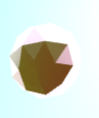
\includegraphics[width=\columnwidth]{zeton.jpg}
\end{center}

Preostanejo še oblaki, ki pa obstajajo le za realističen pridih. Niso ovire in hkrati letalu nič ne doprinesejo. Letalo lahko za zabavo leti skozi njih.
\begin{center}
     \includegraphics[width=\columnwidth]{Oblak.jpg}
\end{center}

Na otoke, oblake in žetone igralec nasploh ne more vplivati zunaj tega, da se v njih z letalom zaleti. 

\section{Uporabniški vmesnik}%done
Uporabnišli vmesnik je precej preprost.V spodnjem levem kotu se nahajajo igralcu pomembni podatki - trenutna hitrost, delež goriva in pa čas igranja. Pred začetkom ire se pojavi tekst "LEFT CLICK TO START", ki podobno, kot tekst ob pavziranju igre "LEFT CLICK TO CONTINUE" zahteva, da za nadaljevanje igre igralec klikne na zaslon, s tem pa se zahteva zaklepanje miške (pointer lock).  

\section{Glasba in zvok}%done
Za zvočne efekte uporabljamo: vesel zvok - ko letalo pobere gorivo, zvok zaleta - ko se letalo zaleti v otok in nadležen piskajoči zvok - ko letalu zmankuje goriva. Dodali smo jih za popestritev. Vse zvoke smo našli na internetu, so royalty-free za takšno in podobno uporabo. Vir zvoka za opozorilo:  \footnote{\url{https://www.https://www.youtube.com/watch?v=R6bpWsyEpbg&ab_channel=SoundLibrary}}, vir zvoka za pobiranje goriva:  \footnote{\url{https://www.youtube.com/watch?v=QRrPiYR6yAw&ab_channel=FastSolution}}, vir zvoka zaleta:  \footnote{\url{https://mixkit.co/free-sound-effects/explosion/}}.


\section{Gameplay}%done
Ko se igra zažene, se na zaslonu izpiše: "LEFT CLICK TO START". Takoj, ko igrale pritisne levo miškino tipko, se poveže z letalom in se začne premikati oz. leteti naprej. Igralec letala ne more ustaviti, z miškinim pogledom ali tipkami WASD ga usmerja po xyz oseh. Če pritisne tipko ESC, se ta povezava prekine, na zaslonu se izpiše: "LEFT CLICK TO CONTINUE", kar da igro na pavzo, letala več ne nadzoruje in spet se lahko z miško premakne ven iz scene v brskalniku. Vsakič, ko pobere žeton, se mu tank goriva napolne za polovico. Žetoni za gorivo se generirajo naključno po svetu. A če se zgenerirajo znotraj kakšnega otoka, se ta žetono zbriše in ponovno se pokliče funkcija za naključno generiranje žetona. Ko se zaleti ali ko mu zmanjka goriva, je igre konec, nima več nadzora nad letalom, izpiše se: "GAME OVER" in število sekund, ki jih je preigral. Za tem mora igro ponovno zagnati in začne na istem mestu, kot prej.
\begin{center}
     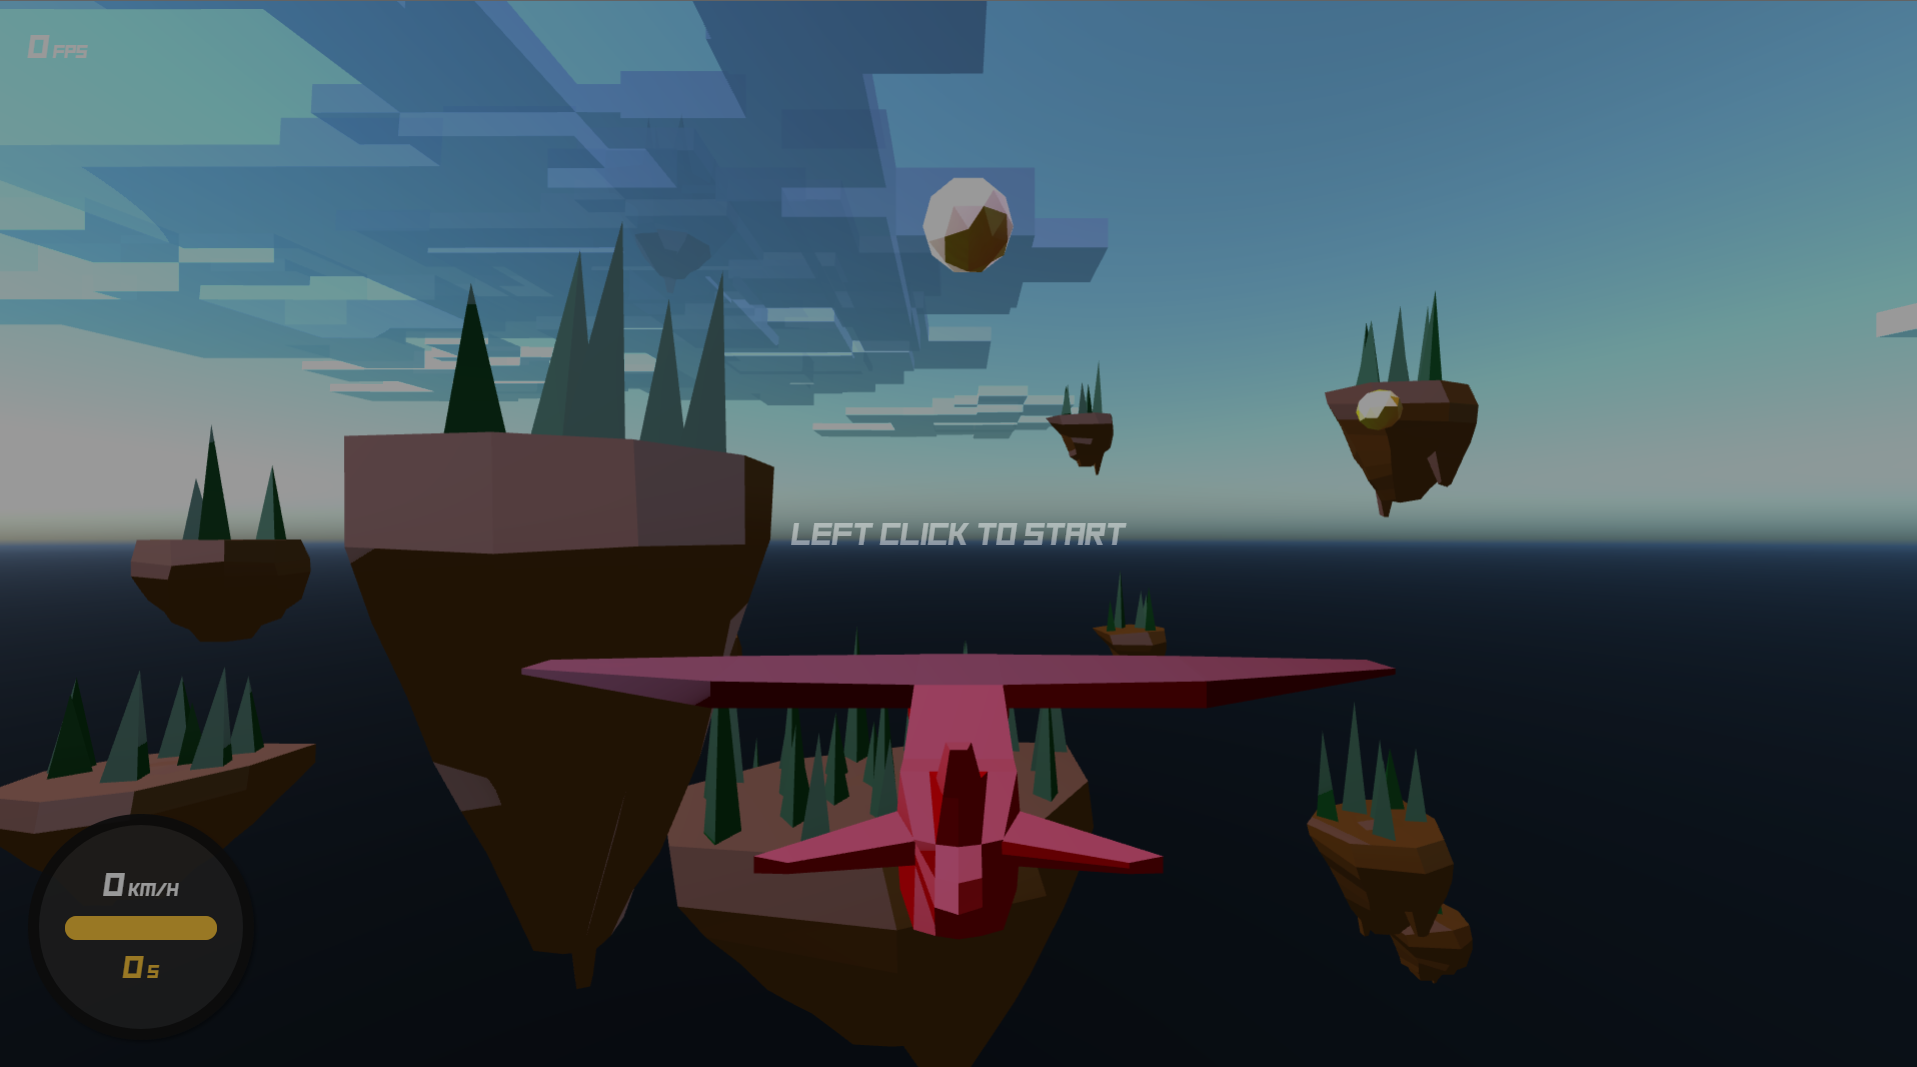
\includegraphics[width=\columnwidth]{start.jpg}
\end{center}

\begin{center}
     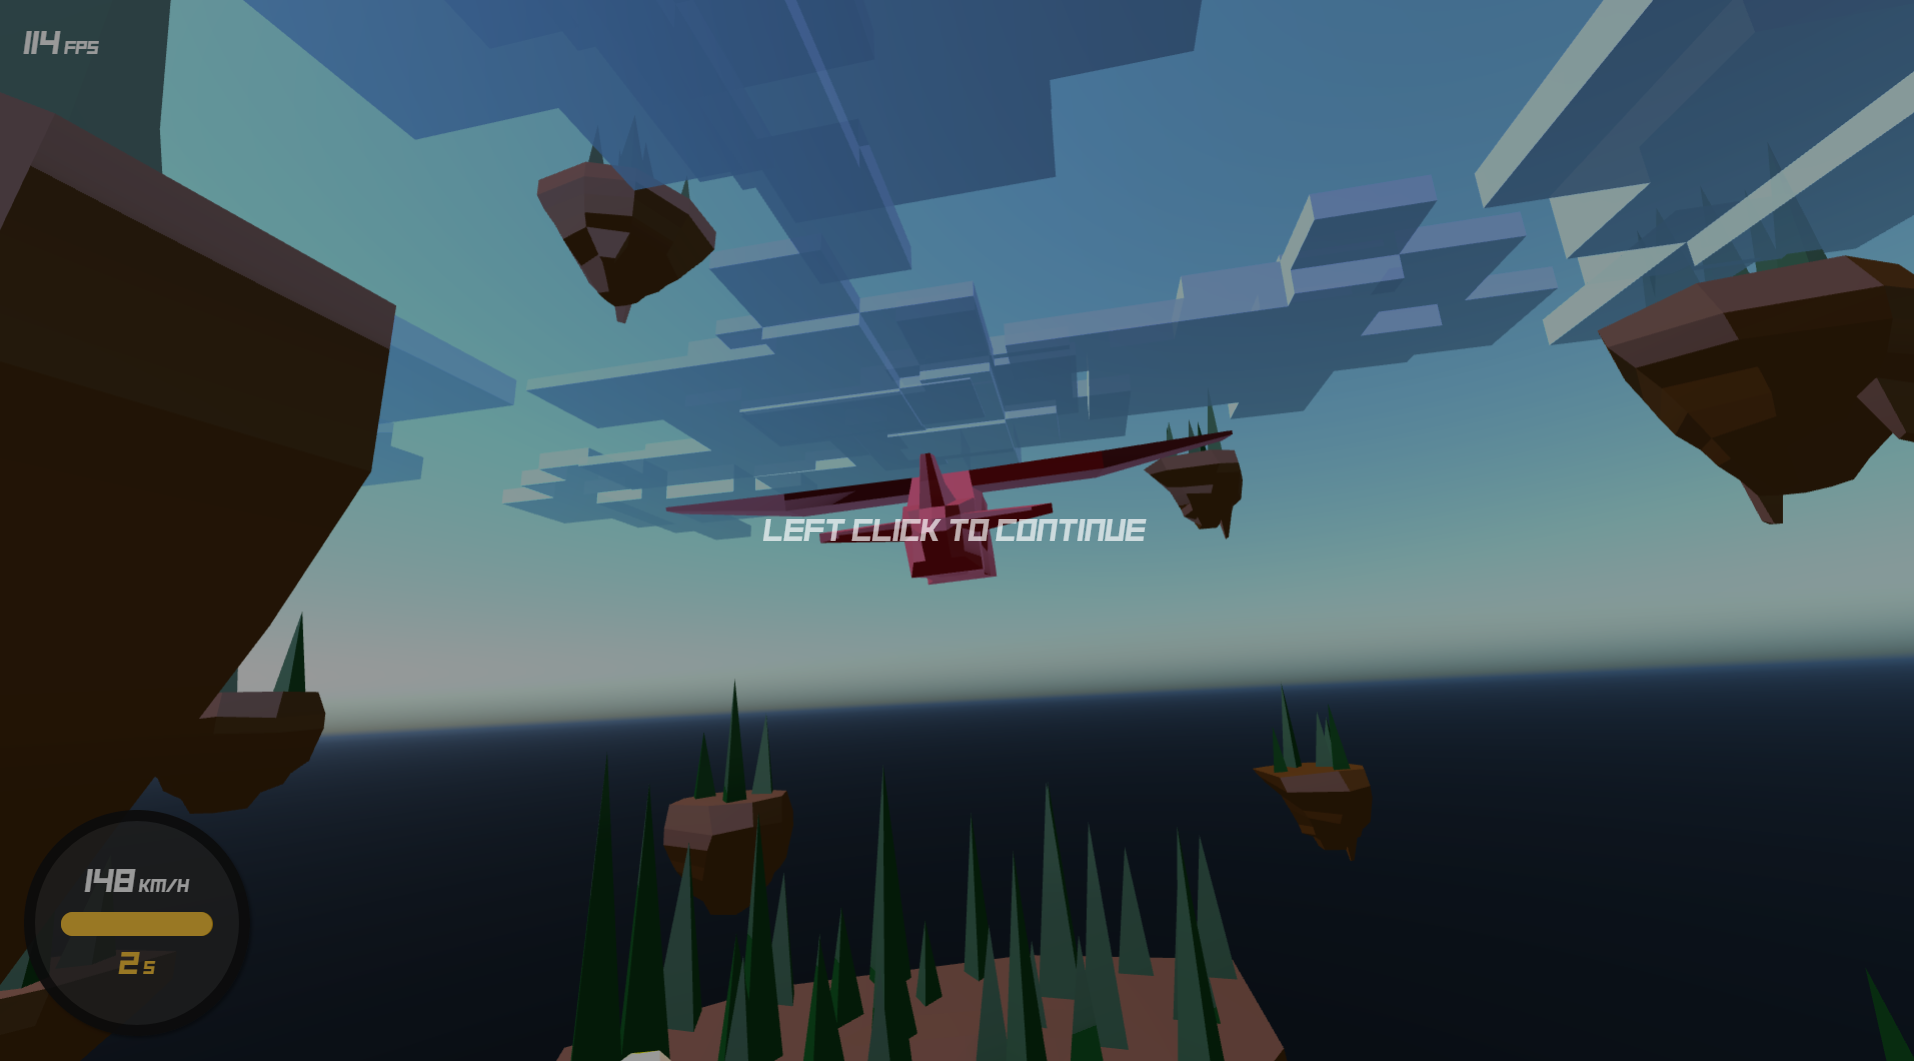
\includegraphics[width=\columnwidth]{continue.jpg}
\end{center}

\begin{center}
     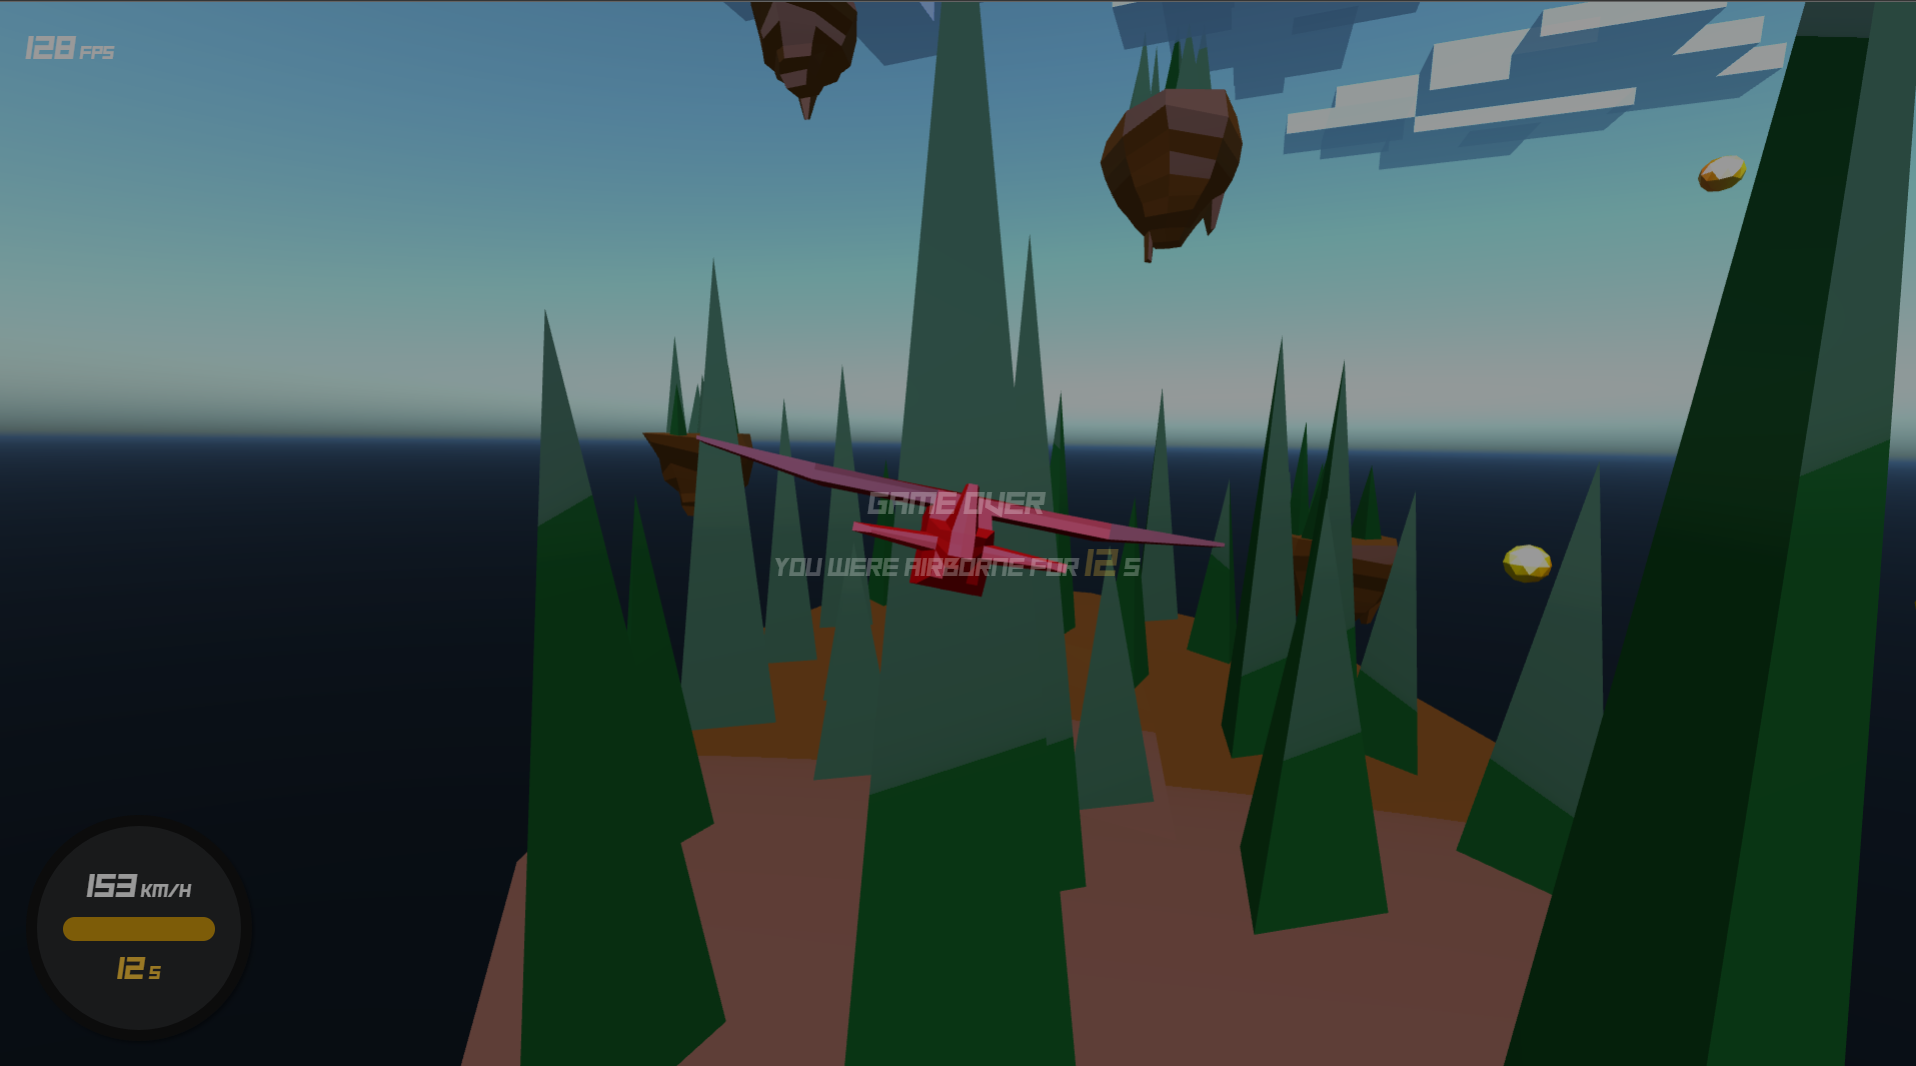
\includegraphics[width=\columnwidth]{game over.jpg}
\end{center}

\section{Tehnični vidiki igre} %done
<<<<<<< HEAD
\subsection{Izris prozornih objektov}%done
=======
\subsubsection{Izris prozornih objektov}%done
>>>>>>> a3e25ab5ae48a05bc5b114d1f26c1c95b2ab919f
Pri izrisu prozornih objektov (oblakov) je pomembno, da jih izrišemo za neprozornimi objekti in urejene po bližini od kamere (najbližje najkasneje).
\subsection{Hitrost in gorivo}%done
Gorivo se na vsakem framu zmanjša za dt * hitrost * konstantna (ki pove, koliko goriva na se porabi na en meter). Hitrost pa se računa, s pomočjo gl-matrix metode vec3.len, ki vrne kvadratni koren seštevka kvadratov.
\subsection{Interpolacija}%done
Za bolj tekoče premikanje letala, kot tudi kamere za njim, linearno interpoliramo rotacije, tako kamere, kot tudi letala, s tem da je rotacija kamere malce hitrejša. Poleg tega pa interpoliramo tudi offset kamere za letalom. 
\subsection{Stanje igre}%done
Za lažjo implementacijo logike igre, smo dodali enume stanja igre (ker jih Javascript direktno ne podpira, smo to implementirali rahlo drugače). Stanja so lahko igrano, pavzirano, konec igre ali začetek. 
<<<<<<< HEAD
\subsection{Naključno generiranje}%done
V igri se na naključnih mestih naključno generirajo tako žetoni, kot oblaki. Poleg tega pa imajo oblaki naključno skaliranje in pa smer premikanja. Pri generiranju žetonov, preverimo, ali se je slučajno zgeneriral znotraj otoka in če se je ponovno pokličemo funkcijo za generiranje žetona, tega pa izbrišemo.
=======
>>>>>>> a3e25ab5ae48a05bc5b114d1f26c1c95b2ab919f

\section{Zaključki in možne nadgradnje} %done
Pri izdelavi smo v praksi utrdili teorijo iz predavanj, se naučili uporabe WebGL-a in senčilnikov, naučili osnove Blenderja ter nadgradili znanje JavaScripta in gita. Predviden scenarij smo uspeli izvesti v celoti, igra pa se v naslednjem projeku v Unityju lahko še nadgradi, doda več objektov (morda nasprotnikov) in predvsem izboljša fizika letenja. Težave so se pojavljale pri kombiniranju logike oz. fizike sveta z glTF objekti. Koristilo bi, da bi na vajah naredili več primerov premikanja ipd. na dejanskih glTF objektih, ne le na preprostih kockastih modelih. 

\small
\bibliographystyle{plain}
%\bibliography{references}

\end{document}
